\graphicspath{{./images/}}

\newcounter{nonFuncReq} %Non functinal requiremet counter
\newcounter{quatar} %Quality target counter

\chapter{Einführung und Ziele}

\section{Business Case}

Die Applikation MEON dient der Registration neuer händler für den mobilen Bezahldienst Paymit (Twint aktuell nicht klar) und zukünftig der Registrierung neuer Handler für Terminal/Acquiring Pakete.  Der Geschäftsprozess ist in der folgenden Grafik vereinfacht dargestellt:

\begin{center}
	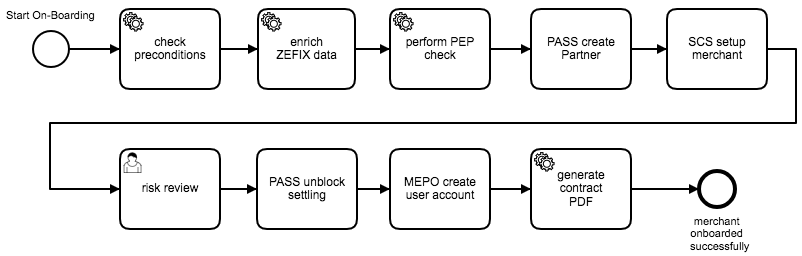
\includegraphics[scale=0.55]{meon-workflow.png}
\end{center}

Die folgende Tabelle beschreibt die einzelnen Teile des Prozesses genauer.

\begin{table}[H]
	\centering
	\caption{Prozessteile}
	\begin{tabular}{ | p{4cm} | p{12cm} | }
		\toprule
		{\textbf{Name}} & {\textbf{Beschreibung}} \\
		\midrule
		Check preconditions & Überprüft ob die Vorbedinungen erfüllt sind. \\ \hline
		enrich ZEFIX data & Reichert die erhaltenen Daten mit den Daten aus dem Handelsregister an. \\ \hline
		perform PEP Check & Prüft ob die Person politisch exponiert ist. \\ \hline
		PASS create partner & Erstellt den Händler (Partner) im Acquering System.\\ \hline
		SCS setup merchant & Registriert den Händler für die Zahlungsterminals. \\ \hline
		risk review  & Risiko Abschätzung im Fall einer politischen exponierten Person. \\ \hline
	    PASS Unblock settling & Schaltet die Verarbeitung von Transaktionen im Acquering System frei. \\ \hline
	    MEPO create user account&  Erstellt einen Account im Kundenportal. \\ \hline
	    generate contract PDF & Generiert ein unterzeichnungsbereits Vertrags PDF.  \\
		\bottomrule
	\end{tabular}
\end{table}

\section{Aufgabenstellung}

Die Architektur der Applikation MEON soll so angepasst werden das Continuous Deployment möglich wird. Damit ist gemeint das jeder Teil der Applikation eigenständig ausgerollt werden kann, ohne andere Komponente herunter zu fahren. Des Weiteren darf der Benutzer nicht von der Änderung betroffen sein respektive seine Anfragen dürfen nicht verloren gehen.
Die Onboarding Anwendung ist funktional komplett implementiert und keine weiteren Anforderungen sind bekannt. Neue funktionale Anforderungen müssen die hier erarbeitete Lösung miteinbeziehen, so dass das Continuous Deployment nicht beeinträchtigt wird.
Die Aufgabe besteht darin die Teile hinsichtlich der Kommunikation von einander zu entkoppeln so das eine Aktualisierung den darin abgebilteten Geschäftsprozess nicht unterbricht.  Der interne Aufbau der Komponenten soll nur angepasst werden falls nötig. 

\section{Anforderungen}

Alle funktionalen Anforderungen sind bereits umgesetzt. Durch die Anpassung der Architektur Richtung Continuous Deployment gibt es aktuell nur nicht funktionale Anforderungen.

\begin{table}[H]
	\centering
	\caption{Nicht funktionale Anforderungen}
	\begin{tabular}{ | p{2cm} | p{14cm} | }
		\toprule
		{\textbf{ID}} & {\textbf{Beschreibung}} \\
		\midrule
		NFA-\arabic{nonFuncReq} \stepcounter{nonFuncReq} & Kunde merkt nicht wenn neue Komponenten der Applikation ausgetauscht werden. \\ \hline
		NFA-\arabic{nonFuncReq} \stepcounter{nonFuncReq} & Verfügbarkeit der Anwendung ist 24x7 (SLA). \\ \hline
		NFA-\arabic{nonFuncReq} \stepcounter{nonFuncReq} & Einhaltung der PCI DSS Anforderung bezüglich Umgang mit Daten resp. deren Zugriffsschutz durch Authentifizierung, Authorisierung und entsprechende Netzwerksegmentierung. \\ \hline
		NFA-\arabic{nonFuncReq} \stepcounter{nonFuncReq} & Die Applikation muss einfach skalierbar sein \\ \hline
		NFA-\arabic{nonFuncReq} \stepcounter{nonFuncReq} & Die Anwendung muss eine hohe Ausfallsicherheit aufweisen \\ \hline
		NFA-\arabic{nonFuncReq} \stepcounter{nonFuncReq} & Bugfixing mittels Vorwärtscommit. Anstelle von Hotfixes wird immer die ganze Applikation neu ausgerollt. \\ \hline
		NFA-\arabic{nonFuncReq} \stepcounter{nonFuncReq} & Die Anwendung lässt sich voll automatisch Ausrollen. \\
		\bottomrule
	\end{tabular}
\end{table}

\subsection{Aspekte}

Die wichtigstens Aspekte der Fachdomäne sind: 
\begin{itemize}
	\item Auswahl eines Paymit Abos
	\item Vertragsabschluss
\end{itemize}

\subsection{Art des Systems}

Bei MEON handelt es sich um ein interaktives Online system.

\subsection{Nutzung des Systems}

\subsection{Schnittstellen}

MEON hat folgende Schnittstellen zu Umsystemen.
\begin{itemize}
	\item PASS: Transaktionsverarbeitungssystem.
	\item SCS:  Verwaltung der Terminal geräte bei den Kunden.
	\item ZEFIX: Handelsregsiteranbindung.
\end{itemize}

\subsection{Datenhaltung}

\begin{itemize}
	\item RDBMS (Presistenz)
\end{itemize}

\section{Qualitätsziele}

Die folgende Tabelle zeigt die wichtigsten Qualitätsziele. Die Szenarien zu den Zielen sind genauer im Kapitel \ref{sec:qualityscenarios} aufgeführt.

\begin{table}[H]
	\centering
	\caption{Qualitätsziele}
	\begin{tabular}{ | p{3cm} | p{13cm} | }
		\toprule
		{\textbf{Name}} & {\textbf{Beschreibung}} \\
		\midrule
		Q-\arabic{quatar} \stepcounter{quatar} & Die neue Architektur soll einfach verständlich und anwendbar sein.\\ \hline
		Q-\arabic{quatar} \stepcounter{quatar} & Die Deployment Pipeline soll einfach wartbar sein. \\ \hline
		Q-\arabic{quatar} \stepcounter{quatar} & Der Benutzer wird durch eine neu Ausrollung der Anwendung nicht beeinträchtigt. \\ \hline
		Q-\arabic{quatar} \stepcounter{quatar} & Die Performanz wird durch die Ausrollung der Applikation nicht beeinträchtigt.\\ 
		\bottomrule
	\end{tabular}
\end{table}

\section{Stakeholder}

\begin{table}[H]
	\centering
	\caption{Stakeholder}
	\begin{tabular}{ | p{3cm} | p{13cm} | }
		\toprule
		{\textbf{Name}} & {\textbf{Beschreibung}} \\
		\midrule
		Business & Repräsentiert die Geschäftstätigkeit der Firma.\\ \hline
		Kunde & Benutzer der Webapplikation. \\ \hline
		Support-Kunde & Support welcher den Kunden bei Problemen unterstützt. \\ \hline
		Legal &  Verantwortlich für die Richtigkeit der Vertragsabschlüsse. \\ \hline
		Risk & Sorgt für die Überprüfung der Personen und der Geschäftstätigkeiten. \\ \hline
		Marketing & Abteilung für den Vertrieb, Werbung, Design. \\ \hline
		Betrieb & Betreibt die Webapplikation auf der Infrastruktur der SIX \\ \hline
		Change Management & Genehmigt Änderungen an der Applikation. \\ \hline
		Entwickler & Setzt die Anforderungen der einzelnen Stakeholder um. \\  \hline
		Unternehmens-architekten & Definieren firmenweite Architekturen und haben den gesamtüberblick über die Applikationslandschaf.\\ 
		\bottomrule
	\end{tabular}
\end{table}
